\documentclass[conference]{IEEEtran}
\IEEEoverridecommandlockouts
% The preceding line is only needed to identify funding in the first footnote. If that is unneeded, please comment it out.
\makeatletter
\def\endthebibliography{%
	\def\@noitemerr{\@latex@warning{Empty `thebibliography' environment}}%
	\endlist
}
\renewcommand{\figurename}{Gambar}
\makeatother
\usepackage{cite}
\usepackage{amsmath,amssymb,amsfonts}
\usepackage{algorithmic}
\usepackage{hyperref}
\usepackage{graphicx}
\usepackage{textcomp}
\usepackage{xcolor}
\usepackage{adjustbox}
\usepackage{multirow}
\usepackage{subcaption}
\def\BibTeX{{\rm B\kern-.05em{\sc i\kern-.025em b}\kern-.08em
		T\kern-.1667em\lower.7ex\hbox{E}\kern-.125emX}}
\begin{document}
	
	\title{Aplikasi Telekardiologi untuk Mobile Android Dilengkapi Sensor ECG}
	
	\makeatletter
	\newcommand{\linebreakand}{%
	\end{@IEEEauthorhalign}
	\hfill\mbox{}\par
	\mbox{}\hfill\begin{@IEEEauthorhalign}
	}
	\makeatother
	
	\author{
		\centering
		
		\IEEEauthorblockN{1\textsuperscript{st}Arief Kurniawan}
		\IEEEauthorblockA{\textit{Departemen Teknik Komputer} \\
			\textit{Fakultas Teknologi Elektro}\\
			\textit{dan informatika Cerdas}\\
			\textit{Institut Teknologi Sepuluh Nopember}\\
			Surabaya, Indonesia 60111 \\
			arifku@te.its.ac.id}
		\and
		\IEEEauthorblockN{2\textsuperscript{nd}I Ketut Eddy Purnama}
		\IEEEauthorblockA{\textit{Departemen Teknik Komputer} \\
			\textit{Fakultas Teknologi Elektro}\\
			\textit{and Informatics Technology}\\
			\textit{Institut Teknologi Sepuluh Nopember}\\
			Surabaya, Indonesia 60111 \\
			fuad@te.its.ac.id}
		\and
		\IEEEauthorblockN{3\textsuperscript{rd} Robby Aldriyanto Raffly }
		\IEEEauthorblockA{\textit{Departemen Teknik Komputer} \\
			\textit{Fakultas Teknologi Elektro}\\
			\textit{and Informatics Technology}\\
			\textit{Institut Teknologi Sepuluh Nopember}\\
			Surabaya, Indonesia 60111 \\
			robby.17072@mhs.its.ac.id}
		
	}
	
	\maketitle
	
	
	\begin{abstract}
		\textit{Jantung merupakan organ yang sangat penting bagi tubuh. Jantung memiliki peran penting yaitu memompa darah ke seluruh bagian tubuh. Apabila terjadi suatu kelainan pada kesehatan jantung maka dapat berakibat fatal dan beresiko kematian. Kematian karena penyakit jantung merupakan salah satu kematian terbanyak di dunia. Penyakit jantung dapat diketahui sejak dini dengan cara memonitoring sinyal detak jantung. Pada Tugas Akhir ini kami mengajukan judul penelitian tentang implementasi sistem telekardiologi. Implementasi sistem telekardiologi yang kami ajukan adalah membuat aplikasi android yang dapat digunakan untuk mengambil data sinyal ECG dari arduino melalui modul bluetooth HC-05. Sinyal ECG tersebut didapatkan arduino dengan menggunakan sensor AD8232. Aplikasi juga memiliki fitur untuk mengirimkan sinyal ECG kepada dokter spesialis jantung sehingga dokter dapat mendiagnosa sinyal ECG pasien tanpa harus mengecek pasien dengan bertemu secara langsung. Aplikasi juga memiliki fitur chat dengan dokter agar pasien dapat berkonsultasi jarak jauh. Aplikasi ini ditujukan untuk pasien penyakit jantung agar disaat kondisi pandemi COVID 19 seperti saat ini pasien tetap dapat berkonsultasi dengan dokter tanpa harus pergi ke Rumah Sakit. Hasil yang diharapkan dari penelitian ini adalah aplikasi dapat mengambil data melalui komunikasi bluetooth, mengirimkan data sinyal ECG kepada dokter, dan chatting.}
		
	\end{abstract}
	\begin{IEEEkeywords}
		\textit{Telekardiologi, ECG}
	\end{IEEEkeywords}
	
	\section{Latar Belakang}
	\IEEEPARstart{T}{elekardiologi} berasal dari kata tele yang berarti jarak jauh dan kardiologi yang merupakan suatu cabang kedokteran yang berhubungan dengan studi dan perawatan kelainan-kelainan di sistem kardiovaskular, yaitu jantung, pembuluh darah, dan pembuluh nadi\cite{cit:1}. Penyakit jantung merupakan penyakit yang menjadi penyebab utama kematian secara global dalam 15 tahun terakhir. Dari 56,9 juta kematian di seluruh dunia pada tahun 2016, lebih dari setengah (54\%) disebabkan oleh 10 penyebab teratas. Penyakit jantung iskemik dan stroke adalah pembunuh terbesar di dunia, yang apabila digabungkan jumlahnya menyebabkan  15,2 juta kematian pada tahun 2016 \cite{cit:2}. Penyakit kardiovaskular juga menjadi penyebab kematian nomor satu di Indonesia. Data dari Institute for Health Metrics and Evaluation, lembaga statistik kesehatan asal Amerika Serikat menyebutkan jumlah kematian akibat penyakit ini mencapai 36,3 persen dari total kematian di Indonesia pada 2016. Selanjutnya, kanker dan diabetes menjadi penyakit yang juga menimbulkan banyak kematian. Indonesia sendiri mendapat peringkat ke-3 di ASEAN setelah Laos dan Filiphine dalam hal jumlah kematian yang disebabkan penyakit kardiovaskular pada tahun 2016 \cite{cit:3}. Salah satu cara untuk mengurangi resiko kematian yang disebabkan penyakit kardiovaskular adalah melakukan pemeriksaan jantung sejak dini. Pemeriksaan kesehatan jantung dapat menggunakan Electrocardiogram (ECG).
	
	
	\vspace{1ex}
	
	Electrocardiogram adalah tes yang menggunakan alat elektrokardiograf yang dapat menunjukkan seberapa cepat jantung seseorang berdetak, dimana denyut jantung tersebut berupa impulse listrik yang diukur oleh sensor. ECG digunakan untuk menampilkan aktivitas pada jantung, sehingga tenaga medis dapat mendiagnosis apakah detak jantung pada pasien tersebut normal atau tidak. Pemeriksaan rekaman ECG biasanya hanya dapat dilakukan
	dilakukan di rumah sakit dengan fasilitas lengkap. Hal tersebut membuat pasien jantung menjadi malas untuk memeriksakan kesehatan jantungnya ke Rumah Sakit. Terlebih lagi disaat kondisi pandemi COVID 19. Rumah Sakit merupakan salah satu tempat yang beresiko menyebabkan penyebaran virus COVID 19. Maka dari itu dibutuhkan sebuah sistem telekardiologi menggunakan aplikasi android agar pasien dan dokter dapat melakukan pemeriksaan secara online tanpa harus pergi ke Rumah Sakit.
	
	\vspace{1ex}
	
	Pemeriksaan rekaman ECG masih dilakukan secara offline di Rumah Sakit. Kondisi pandemi COVID 19 menyebabkan Rumah Sakit menjadi tempat yang beresiko penyebaran virus. Oleh karena itu, dibutuhkan sistem telekardiologi dengan menggunakan aplikasi android yang dapat digunakan pasien untuk mengambil sinyal ECG dan mengirim data sinyal ECG kepada dokter spesialis sehingga pasien dapat berkonsultasi dirumah pribadi.
	
	\vspace{1ex} 
	
	 Penelitian yang terkait dengan judul yang kami ajukan adalah "IoT based Real Time ECG Monitoring System
	using Cypress WICED". (Uttam U. Deshpande, Milan A. Kulkarni)\cite{cit:4}.Penelitian ini merancang dan menerapkan sistem pemantauan ECG berdasarkan Cypress Wireless Internet Connectivity for Embedded Devices (WICED) dan membandingkannya dengan  Wi-Fi, Bluetooth, Zigbee dan BLE untuk membuktikan kecepatannya mengirim data yang lebih tinggi dan memiliki cakupan area yang lebih luas. Selain itu juga ada penelitian terkait yang berjudul "An IoT-cloud Based Wearable ECG Monitoring System
	for Smart Healthcare". (Zhe Yang, Qihao Zhou, Lei Lei, Kan Zheng, Wei Xiang)\cite{cit:5}.\ Penelitian ini merancang dan menerapkan sistem pemantauan EKGberdasarkan teknik IoT cloud. Penetian ini juga menggunakan Wi-Fi, Bluetooth, Zigbee dan BLE untuk mengirim data ke cloud. Cloud IoT bertanggung jawab untuk memvisualisasikan data EKG kepada pengguna dan menyimpan data untuk analisis lebih lanjut, yang diimplementasikan atas dasar tiga server, yaitu server HTTP, Server MQTT, dan server penyimpanan.
	
	\section{Desain dan Implementasi}
	\vspace{1ex}
	Penelitian ini merupakan penerapan dari bidang \textit{Mobile Programming} dan \textit{Internet of Things} yang berjutuan untuk membangun sistem monitoring detak jantung pasien serta agar pasien jantung dapat berkonsultasi dengan dokter spesialis melalui aplikasi android. Gambar \ref{Gambar:1} merupakan arsitektur dan blok diagram alur kerja sistem. Aplikasi android menjadi dapat mengambil data sinyal jantung pasien yang telah dideteksi oleh sensor AD8232 melalui modul bluetooth HC-05. Aplikasi dapat mengirimkan data sinyal jantung pasien kepada dokter spesialis serta terdapat fitur chatting agar pasien dapat berkonsultasi dengan dokter. 
	\vspace{1ex}
	\begin{figure}[!ht] \centering
		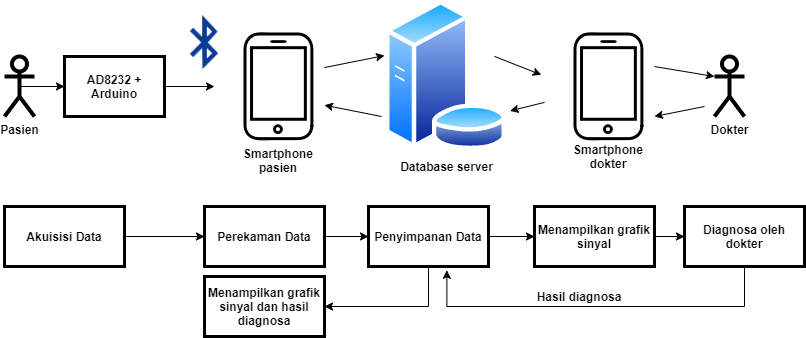
\includegraphics[width=0.47\textwidth]{img/arsitektur.png}
		\caption{Arsitektur dan blok diagram sistem}
		\label{Gambar:1}
	\end{figure}
	\vspace{1ex}
	
	Gambar diatas menunjukkan mengenai alur kerja sistem. Sistem memiliki empat tahap utama yaitu akuisisi data, perekaman data, penyimpanan data, dan diagnosa data.
	
	\vspace{1ex}
	
	
	

	
	
	\subsection{Desain UI Aplikasi}
	\vspace{1ex}
	Aplikasi android memiliki 2 desain yaitu untuk dokter dan
	pasien. Desain UI aplikasi untuk pasien memiliki fitur tambahan. Pada aplikasi pasien memiliki fitur untuk merekam sinyal
	ECG sedangkan pada aplikasi dokter tidak disediakan fitur tersebut. Desain aplikasi dokter
	ditunjukkan pada Gambar \ref{fig:3.2}. Sedangkan desain UI untuk pasien ditunjukkan pada Gambar \ref{fig:3.3}. 
	
	\begin{figure}[!ht] \centering
		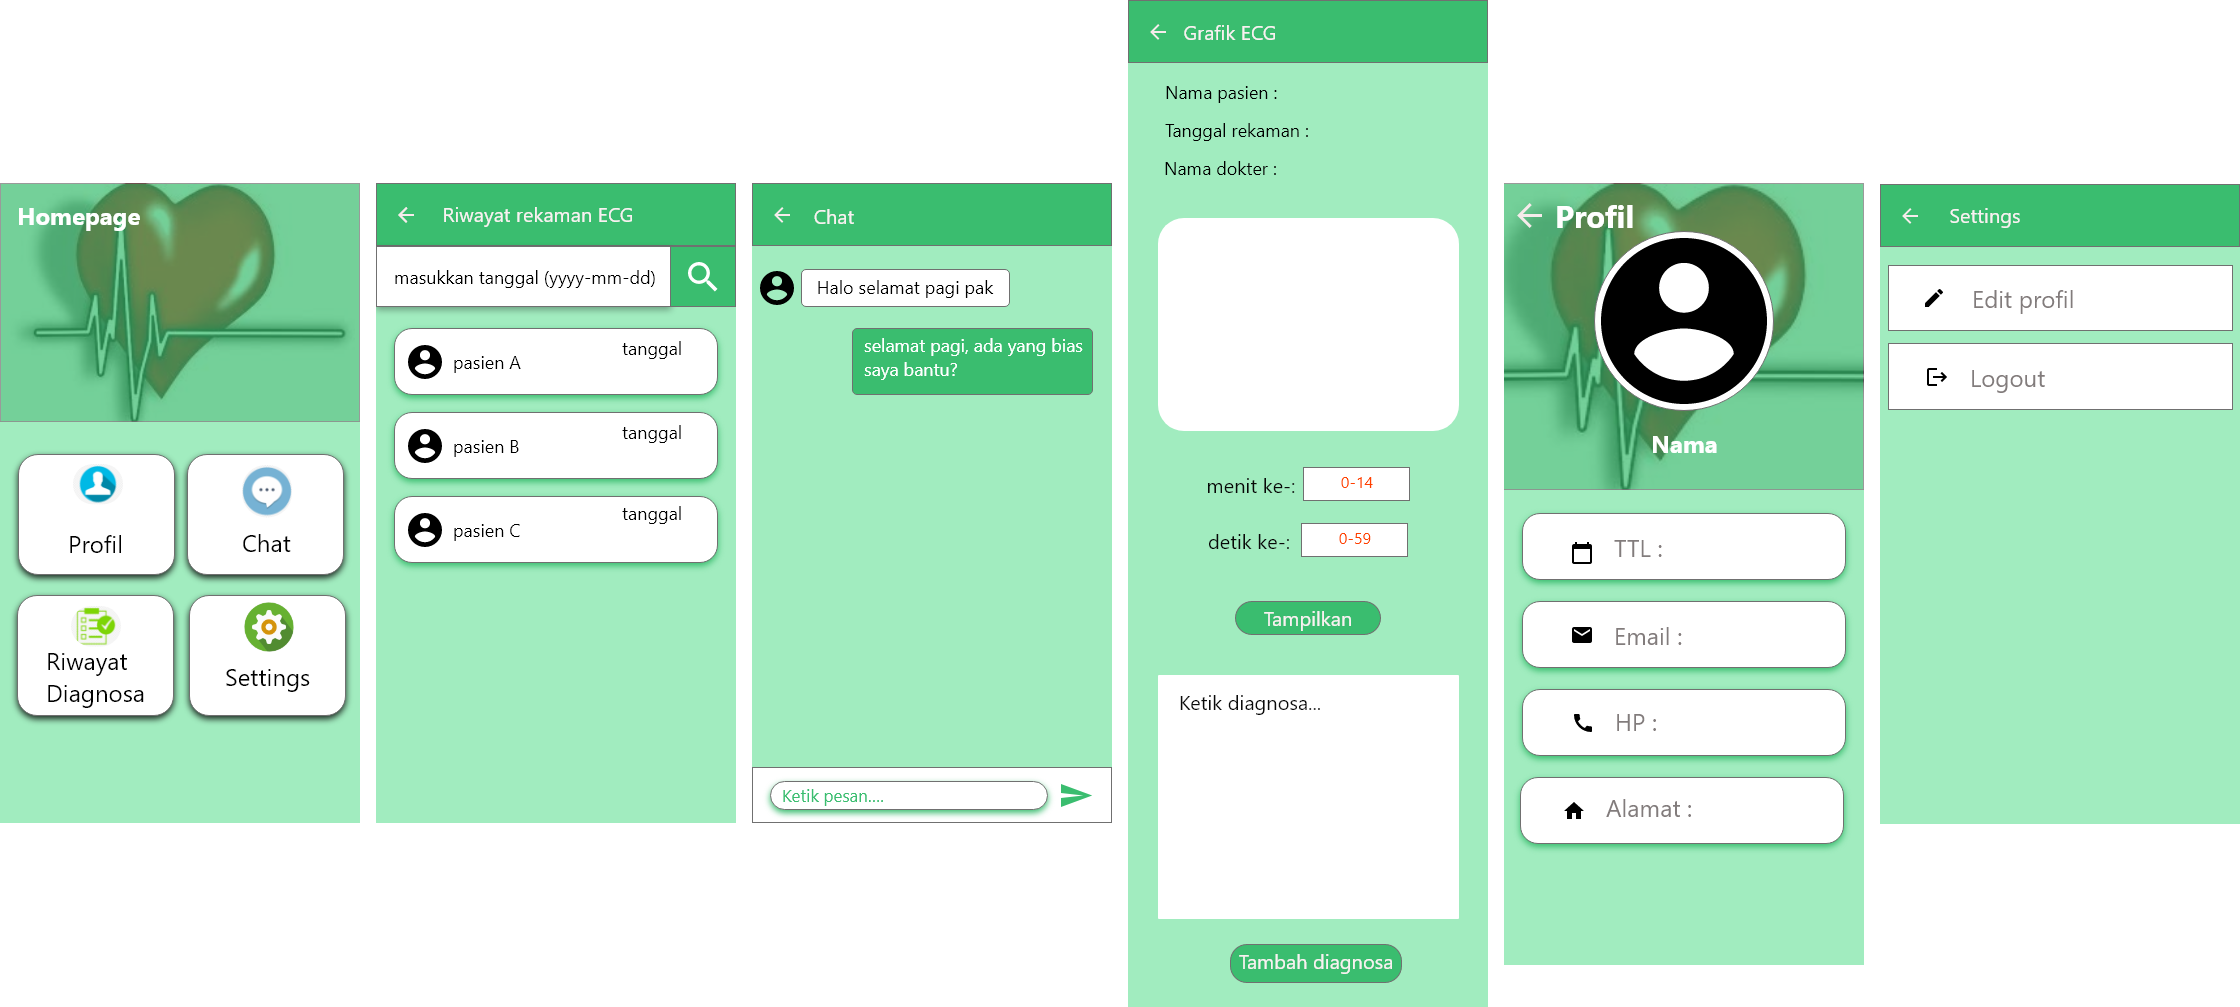
\includegraphics[width=0.47\textwidth]{img/dokterUI.png}
		\caption{Desain UI pada aplikasi dokter.}
		\label{fig:3.2}
	\end{figure}
	\begin{figure}[!ht] \centering
		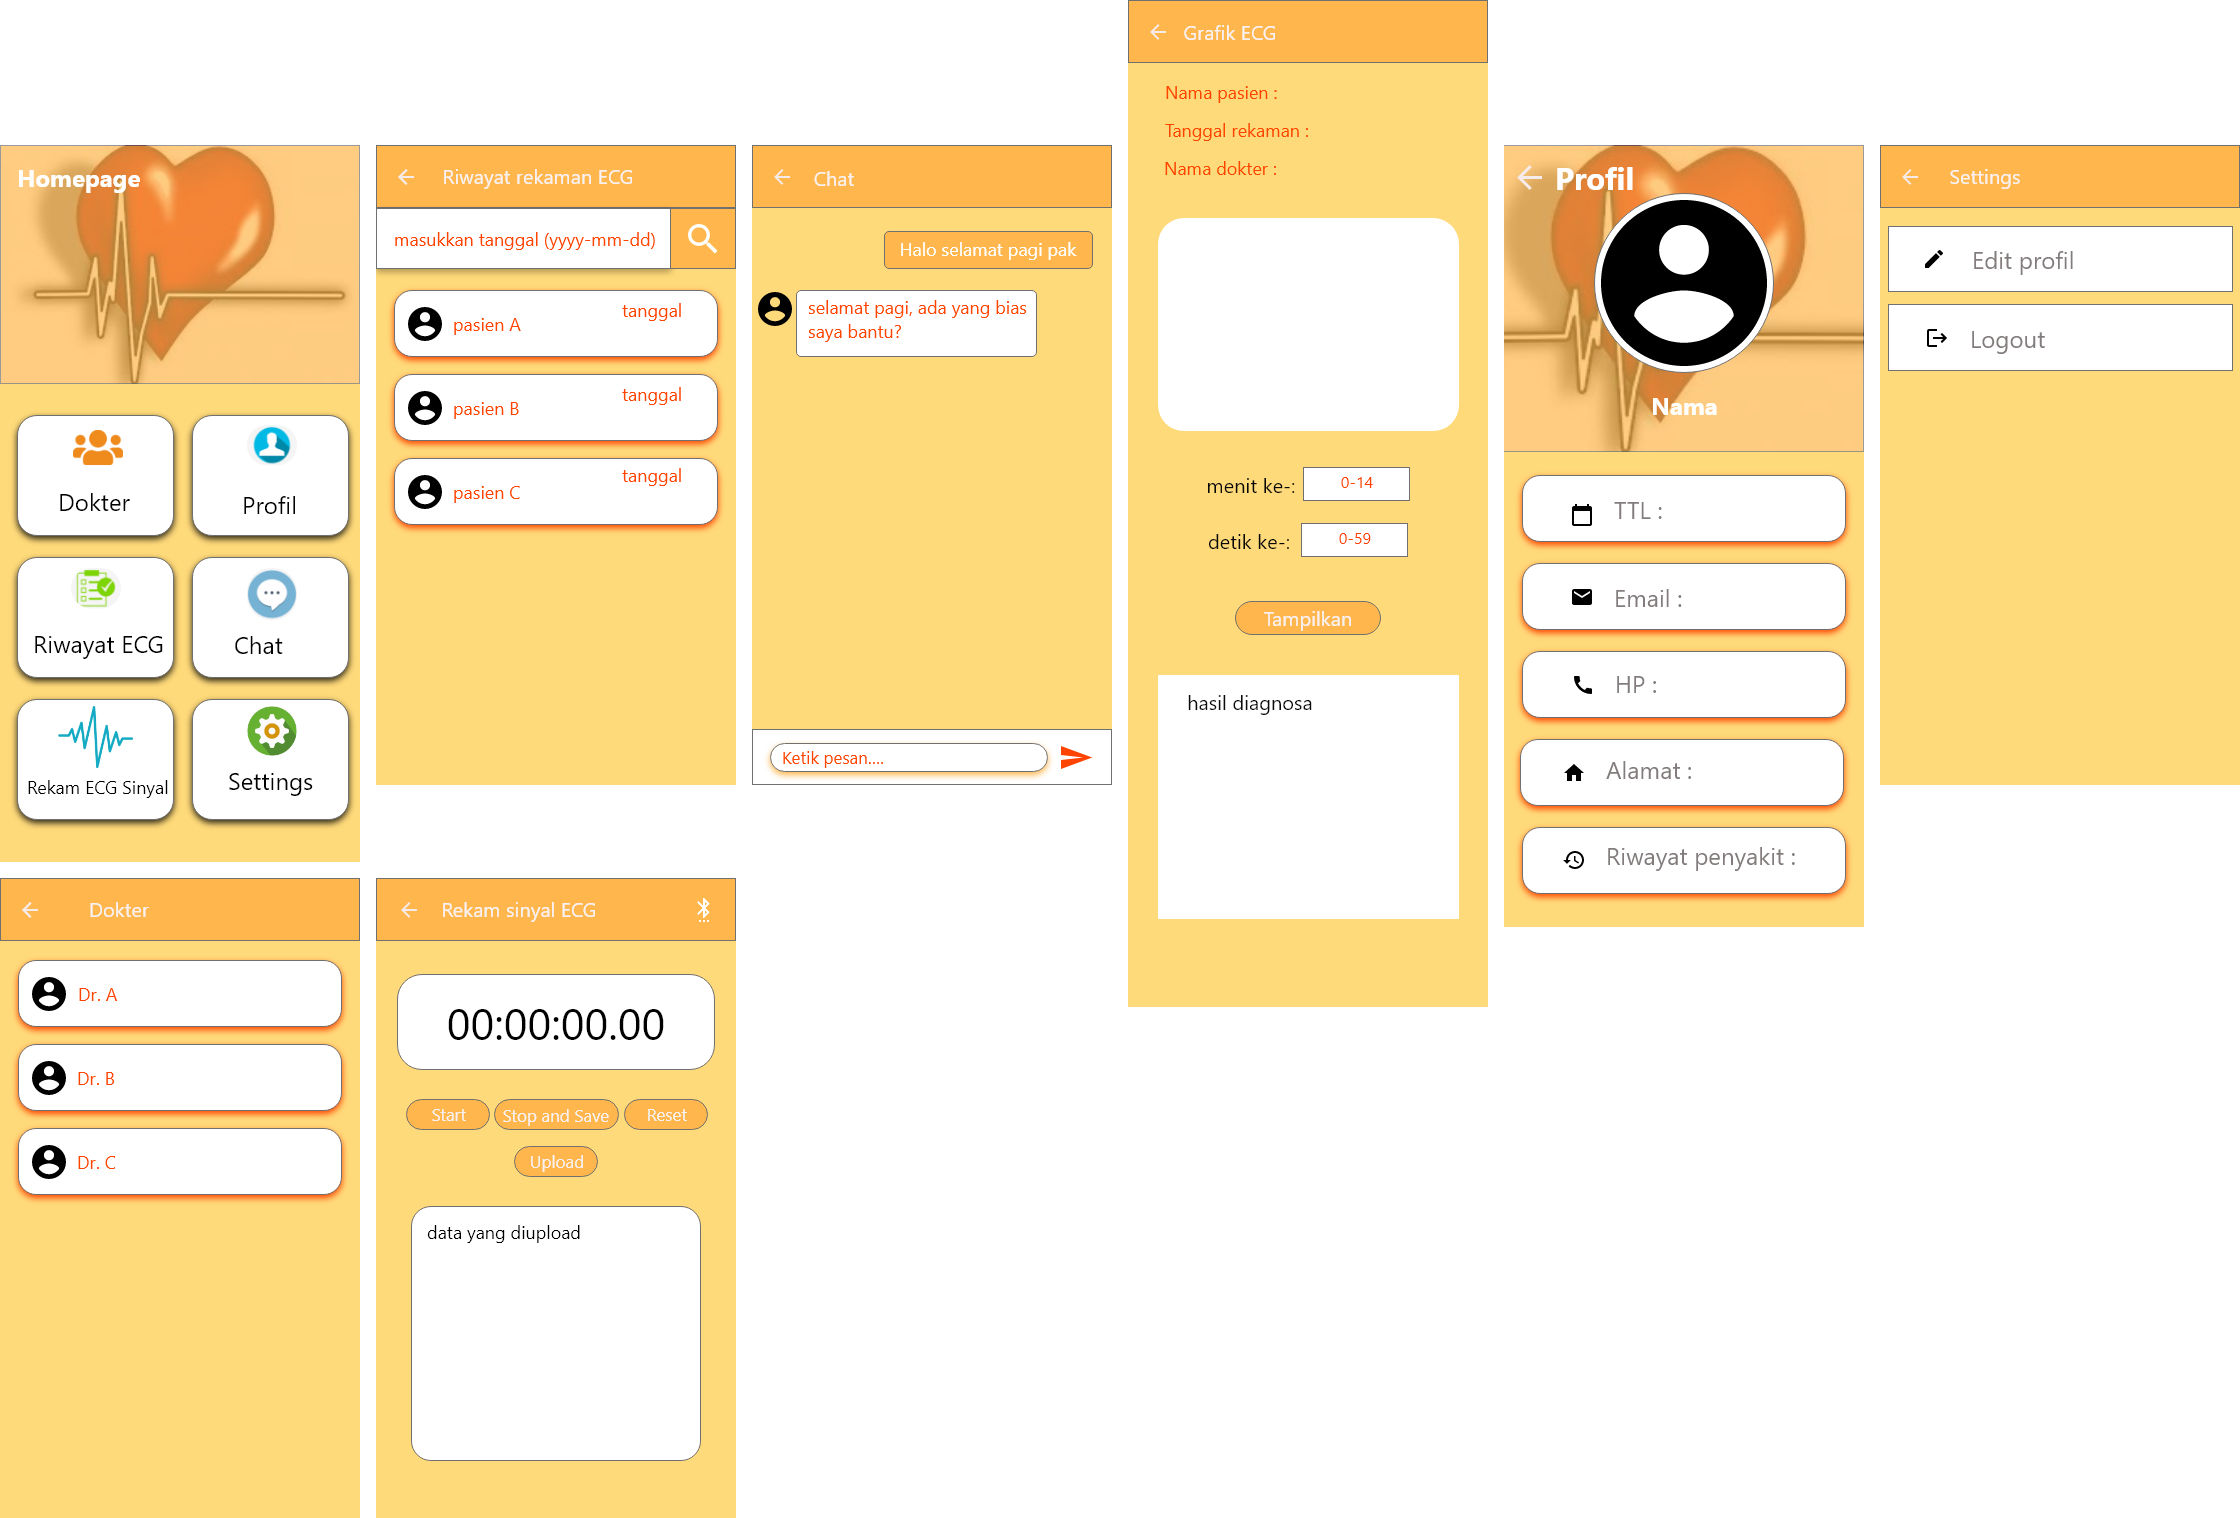
\includegraphics[width=0.47\textwidth]{img/pasienUI.png}
		\caption{Desain UI pada aplikasi pasien.}
		\label{fig:3.3}
	\end{figure}
	\vspace{1ex}
	Pada kedua gambar tersebut terdapat
	sedikit perbedaan desain antara milik dokter dengan pasien. Perbedaan pertama desain tersebut terdapat pada jumlah menu di homepage. Pada desain UI homepage milik dokter memiliki menu yang lebih sedikit daripada pasien, hal ini dikarenakan dokter tidak perlu menggunakan fitur rekam sinyal sinyal dan juga fitur melihat dokter lain. Perbedaan kedua terdapat
	pada layar grafik ECG yang berguna dapat menampilkan grafik sinyal jantung pada menit dan detik tertentu sesuai keinginan user.
	Perbedaan pada layar grafik ECG adalah pada layar dokter
	terdapat form dan tombol untuk menambahkan diagnosa sedangkan pada layar pasien hanya membutuhkan hasil diagnosa.
	
	\vspace{1ex}
	
	\subsection{Desain Database}
	\vspace{1ex}
	
	Pada penelitian ini kami menggunakan database MySQL. Dalam database terdapat 4 tabel yang diperlukan untuk menyimpan masing-masing data, yaitu:
	\begin{enumerate}
		\vspace{1mm}
		\item Tabel data\_ecg, memiliki 10 kolom, 1 kolom merupakan foreign key dari tabel data\_diagnosa. Tabel data\_ecg digunakan untuk menyimpan data rekaman sinyal jantung pasien yang mana akan dapat ditampilkan pada aplikasi android.
		\vspace{1mm}
		\item Tabel data\_diagnosa, memiliki 4 kolom, Tabel ini digunakan sebagai tempat penyimpanan hasil diagnosa yang telah ditambahkan oleh dokter.
		\vspace{1mm}
		\item Tabel user, memiliki 10 kolom. Tabel user digunakan sebagai tempat menyimpan data pengguna aplikasi, baik data dari dokter maupun pasien disimpan dalam tabel ini.
		\vspace{1mm}
		\item Dan tabel data\_chat yang memiliki 5 kolom. Tabel data\_chat diperlukan untuk menyimpan data chat antara pasien dan dokter.
	\end{enumerate}
	
	Berikut merupakan desain database pada penelitian ini ditunjukkan pada Gambar \ref{fig:3.4}. 
	\begin{figure}[!ht] \centering
		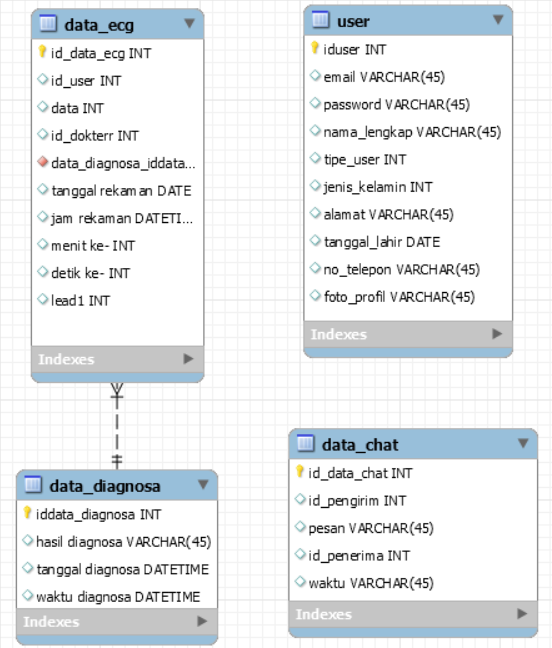
\includegraphics[width=0.47\textwidth]{img/db.png}
		\caption{Desain database.}
		\label{fig:3.4}
	\end{figure}
	\vspace{1ex}
	
	\subsection{Akuisisi Data}
	\vspace{1ex}
	Data sinyal ECG diambil menggunakan modul AD8232. AD8232 adalah blok pengkondisian sinyal terintegrasi untuk Electrocardiogram (ECG) dan aplikasi pengukuran biopotensial lainnya. AD8232 dirancang agar dapat mengekstrak, memperkuat, dan memfilter sinyal biopotensial kecil di hadapan kondisi bising, seperti suara yang dibuat oleh gerakan tubuh. Modul AD8232 memiliki sembilan pin, yaitu SDN, LO +, LO-, OUTPUT, 3.3V, GND, dan juga disediakan pin RA (Lengan Kanan), LA (Lengan Kiri), dan RL (Kaki Kanan) yang dapat dihubungkan dengan tambahan sensor AD8232 yang lain untuk membuat custom jumlah leadnya. Selain itu, modul AD8232 memiliki lampu indikator LED yang akan berkedip mengikuti irama detak jantung\cite{cit:6}.
	Berikut ini merupakan gambar modul AD8232.
	\vspace{1ex}
	\begin{figure}[!ht] \centering
		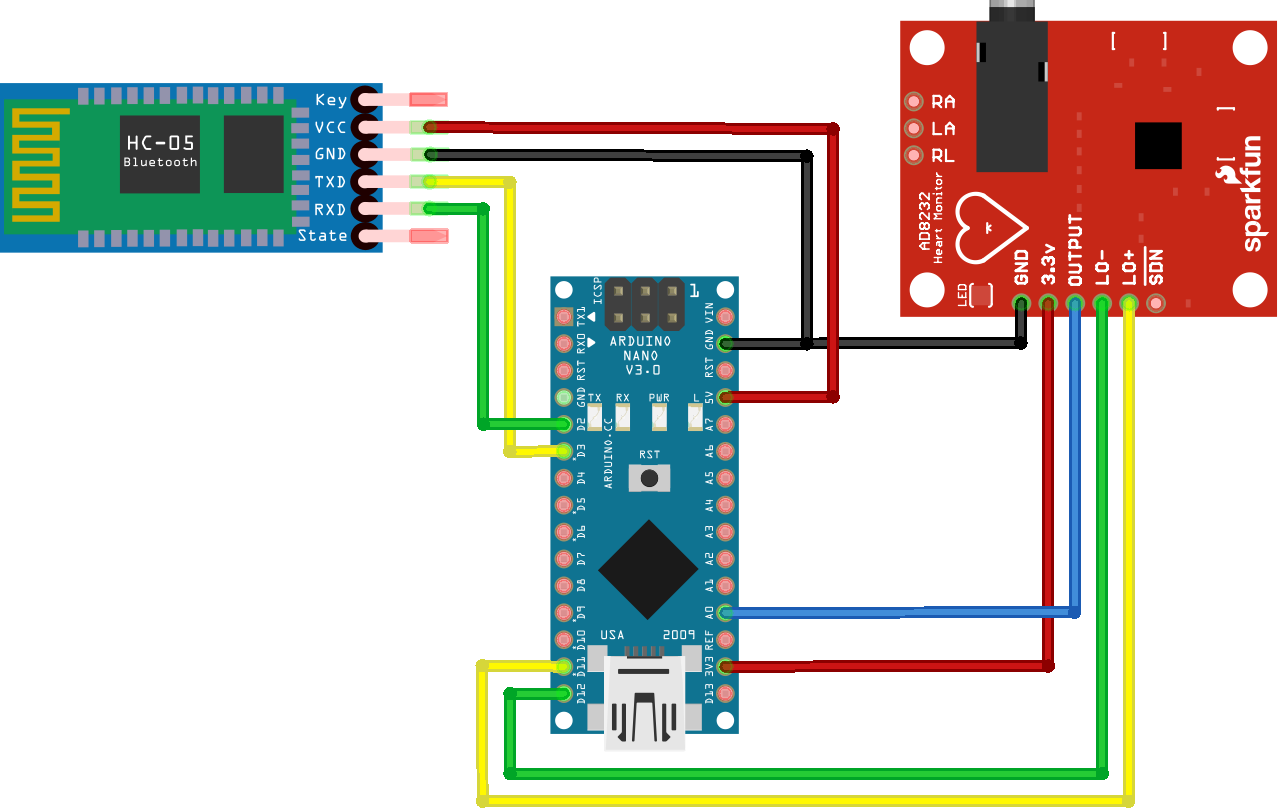
\includegraphics[width=0.47\textwidth]{img/desainperangkat.png}
		\caption{Desain perangkat ECG}
		\label{Gambar:2}
	\end{figure}
	\vspace{1ex}
	Akuisisi data dilakukan dengan frekuensi data 100 Hz yaitu 100 data setiap detik. Data yang diterima arduino dikirim menuju aplikasi menggunakan modul bluetooth HC-05.
	
	\subsection{Perekaman Data}
	\vspace{1ex}
	Perekaman data dilakukan oleh aplikasi android. Proses rekaman pada pasien adalam kurang dari sampai dengan 15 menit.   Berikut merupakan implementasi halaman rekaman data pada aplikasi android ditunjukkan oleh Gambar \ref{fig:3.5}.
	
	\begin{figure}[h] \centering
		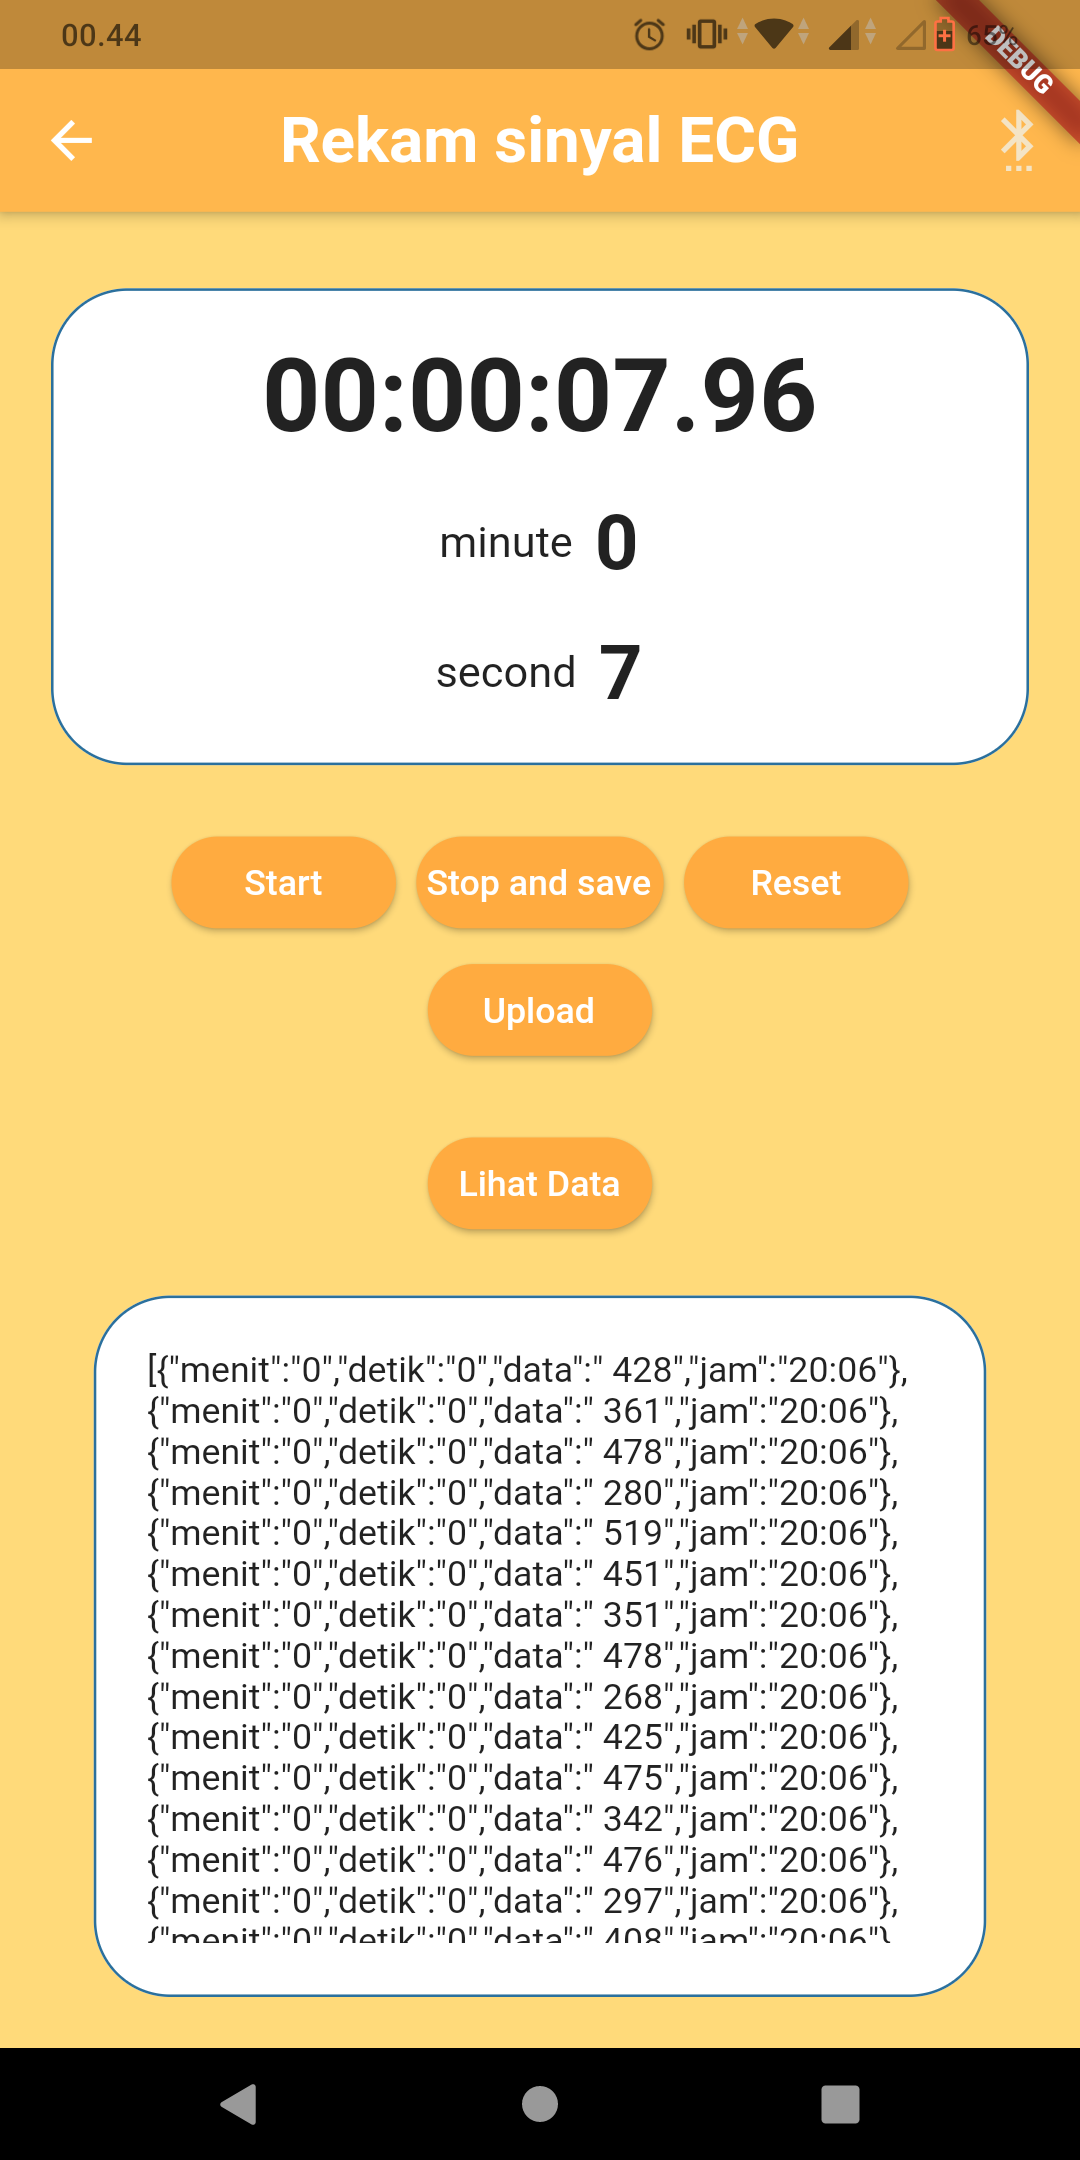
\includegraphics[width=0.2\textwidth]{img/layar_rekaman.png}
		\caption{Implementasi UI Rekam Sinyal ECG.}
		\label{fig:3.5}
	\end{figure}
	
	Selama proses rekaman berlangsung, aplikasi akan menerima data sinyal terus-menerus dari modul bluetooth HC-05. Aplikasi akan menyimpan data sinyal kedalam string saat proses rekaman berlangsung. Setelah rekaman selesai, aplikasi akan menyimpan data sinyal dari variabel string kedalam file.txt. Dapat dilihat pada layar rekaman (Gambar \ref{fig:3.5}) terdapat stopwatch untuk mengetahui seberapa lama telah melakukan rekaman. Pada layar ini terdapat 4 tombol, yaitu tombol Start yang berfungsi untuk memulai rekaman, Stop and Save berfungsi untuk menghentikan rekaman dan menyimpan data dalam file.txt, tombol Reset berfungsi untuk mengembalikan stopwatch dengan keadaan waktu 00:00:00.00, tombol Upload yang berguna untuk mengupload data sinyal menuju database, dan yang terakhir adalah tombol Lihat Data yang berguna untuk menampilkan isi dari file.txt. Isi file.txt ditampilkan pada box putih seperti yang tertera dibawah tomboh Lihat Data.
	
	\vspace{1ex} 
	\subsection{Penyimpanan Data}
	\vspace{1ex}
	Data rekaman sinyal  ECG yang diupload oleh aplikasi pada database disimpan dalam tabel data\_ecg. Data ECG disimpan beserta atribut lainnya sesuai kolom yang ada pada tabel data\_ecg. 
	Berikut merupakan potongan database pada tabel data\_ecg yang ditunjukkan pada Gambar  \ref{fig:3.6}.
	
	\begin{figure}[h] \centering
		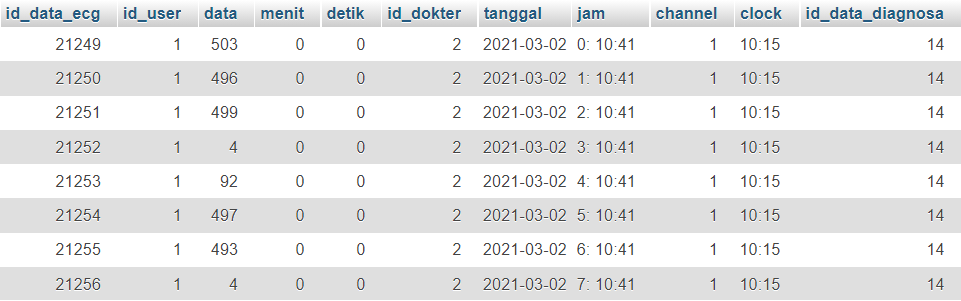
\includegraphics[width=0.47\textwidth]{img/tabel data ecg.png}
		\caption{Tabel data\_ecg.}
		\label{fig:3.6}
	\end{figure}
	
	\vspace{1ex} 
	\subsection{Menampilkan Data}
	\vspace{1ex}
	
	Data yang telah disimpan pada database yaitu dalam tabel data\_ecg dapat diambil oleh aplikasi dokter dan pasien untuk ditampilkan dalam bentuk grafik. Pada screen grafik ECG, pengguna dapat melihat data ECG sesuai dengan waktu yang ditentukan yaitu pada (menit awal, detik awal) sampai dengan (menit akhir, detik akhir) dengan selisih waktu detik yang dapat diatur pada box (parameter range). Pengguna juga dapat melihat data selanjutnya dengan menekan tombol "selanjutnya" serta dapat kembali ke data sebelumnya dengan menakan tombol "sebelumnya". Berikut adalah tampilan dari screen Grafik sinyal ECG dokter ditunjukkan pada Gambar \ref{fig:3.7}. 
	
	\begin{figure}[h] \centering
		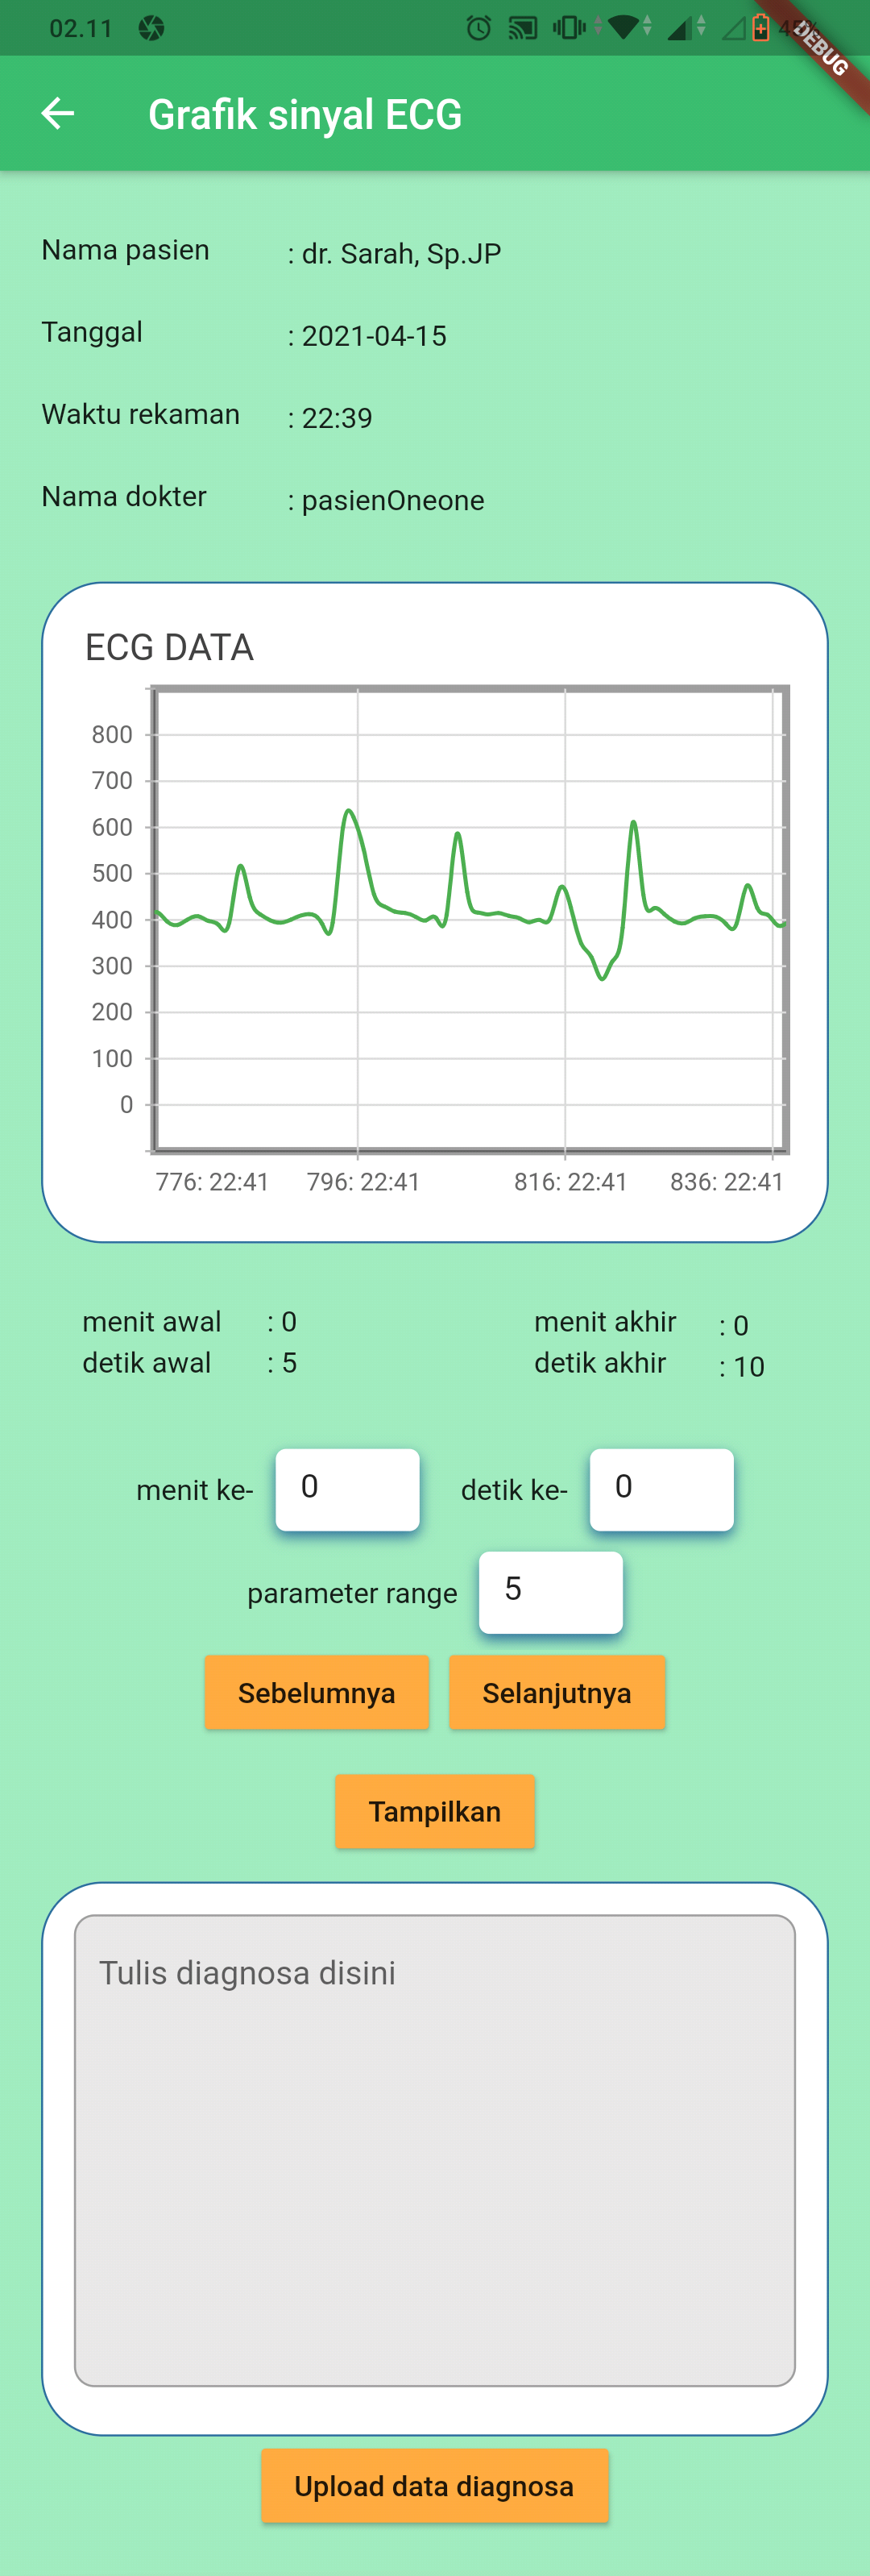
\includegraphics[width=0.2\textwidth]{img/layar_grafikECGdokter.png}
		\caption{Implementasi UI Grafik ECG dokter.}
		\label{fig:3.7}
	\end{figure}
	
	Pada grafik tersebut terdiri dari sumbu X dan sumbu Y. Sumbu X merupakan data ECG yang diambil dari kolom data pada tabel data\_ecg, sedangkan sumbu Y merupakan data dari kolom jam pada tabel data\_ecg (Gambar \ref{fig:3.6}). Untuk tampilan Grafik sinyal ECG pasien tidak jauh berbeda. Berikut adalah tampilan dari screen Grafik sinyal ECG pasien ditunjukkan pada Gambar \ref{fig:3.8}.
	
	\begin{figure}[h] \centering
		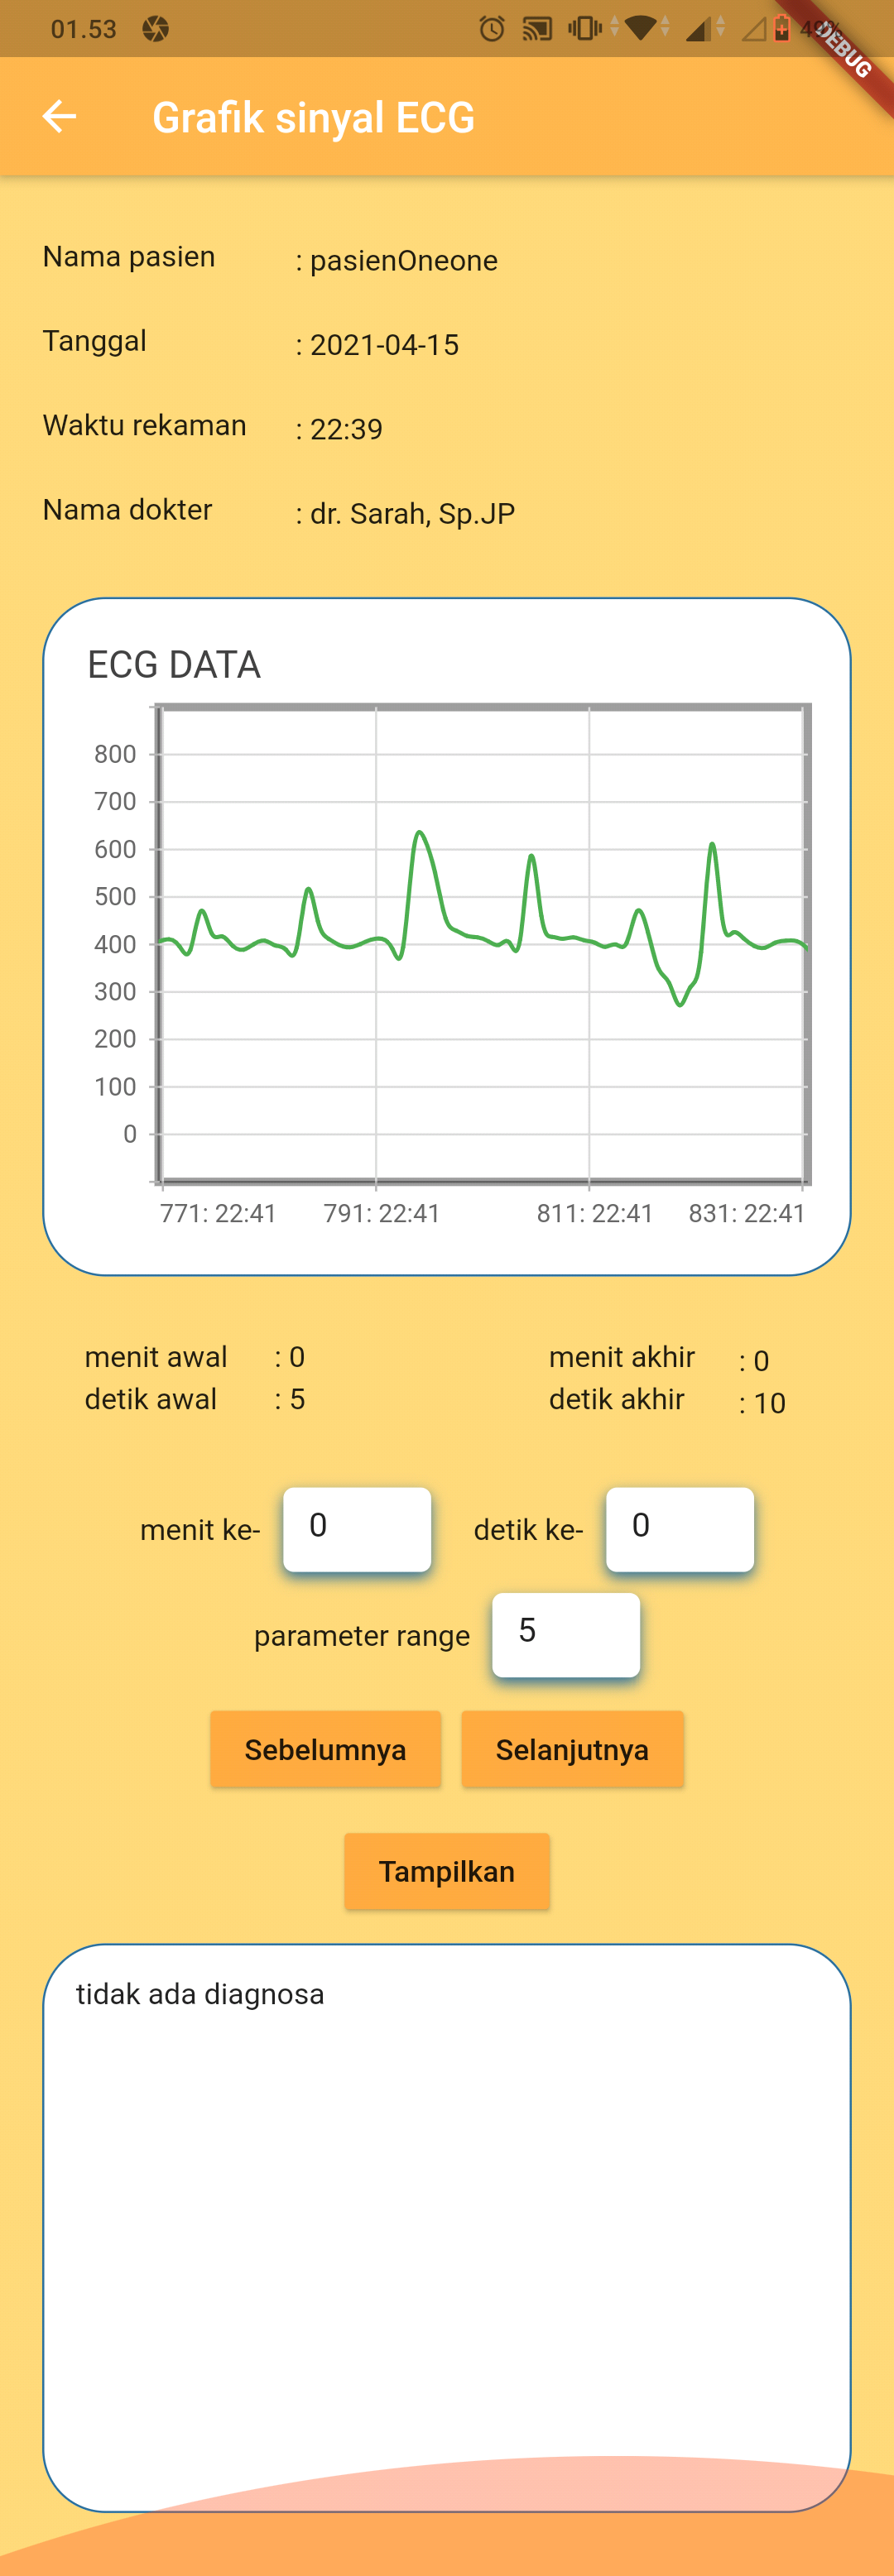
\includegraphics[width=0.2\textwidth]{img/layar_grafikECGpasien.png}
		\caption{Implementasi UI Grafik ECG pasien.}
		\label{fig:3.8}
	\end{figure}
	
	Dapat dilihat pada screen dokter (Gambar \ref{fig:3.7}) terdapat box berwarna abu-abu dengan keterangan "Tulis diagnosa disini" yang berarti pada screen dokter dapat ditambahkan diagnosa melalui box tersebut dan kemudian diupload dengan cara menekan tombol "Upload data diagnosa". Sedang kan pada screen pasien (Gambar \ref{fig:3.8}) hanya terdapat box putih tanpa ada tombol upload data diagnosa. Box putih tersebut adalah tempat hasil diagnosa yang diberikan oleh dokter.
	
	\vspace{1ex} 
	\subsection{Diagnosa Data}
	\vspace{1ex}
	
	Diagnosa sinyal ECG dilakukan secara manual yaitu oleh dokter. Dokter dapat menambahkan diagnosa pada rekaman ECG pasien dimenit dan detik tertentu, dapat dilihat pada Gambar \ref{fig:3.7} sebelumnya. Pada screen tersebut terdapat box untuk dokter yang berfungsi untuk tempat menambahkan diagnosa. Setelah dokter selesai menambahkan diagnosa, kemudian dapat mengupload ke database melalui tombol "Upload data diagnosa". Diagnosa yang telah diupload ke database akan disimpan pada tabel data\_diagnosa. Kemudian data diagnosa dapat ditampilkan pada aplikasi smarftphone pasien seperti yang ditunjukkan Gambar \ref{fig:3.9}.
	
	\begin{figure}[h] \centering
		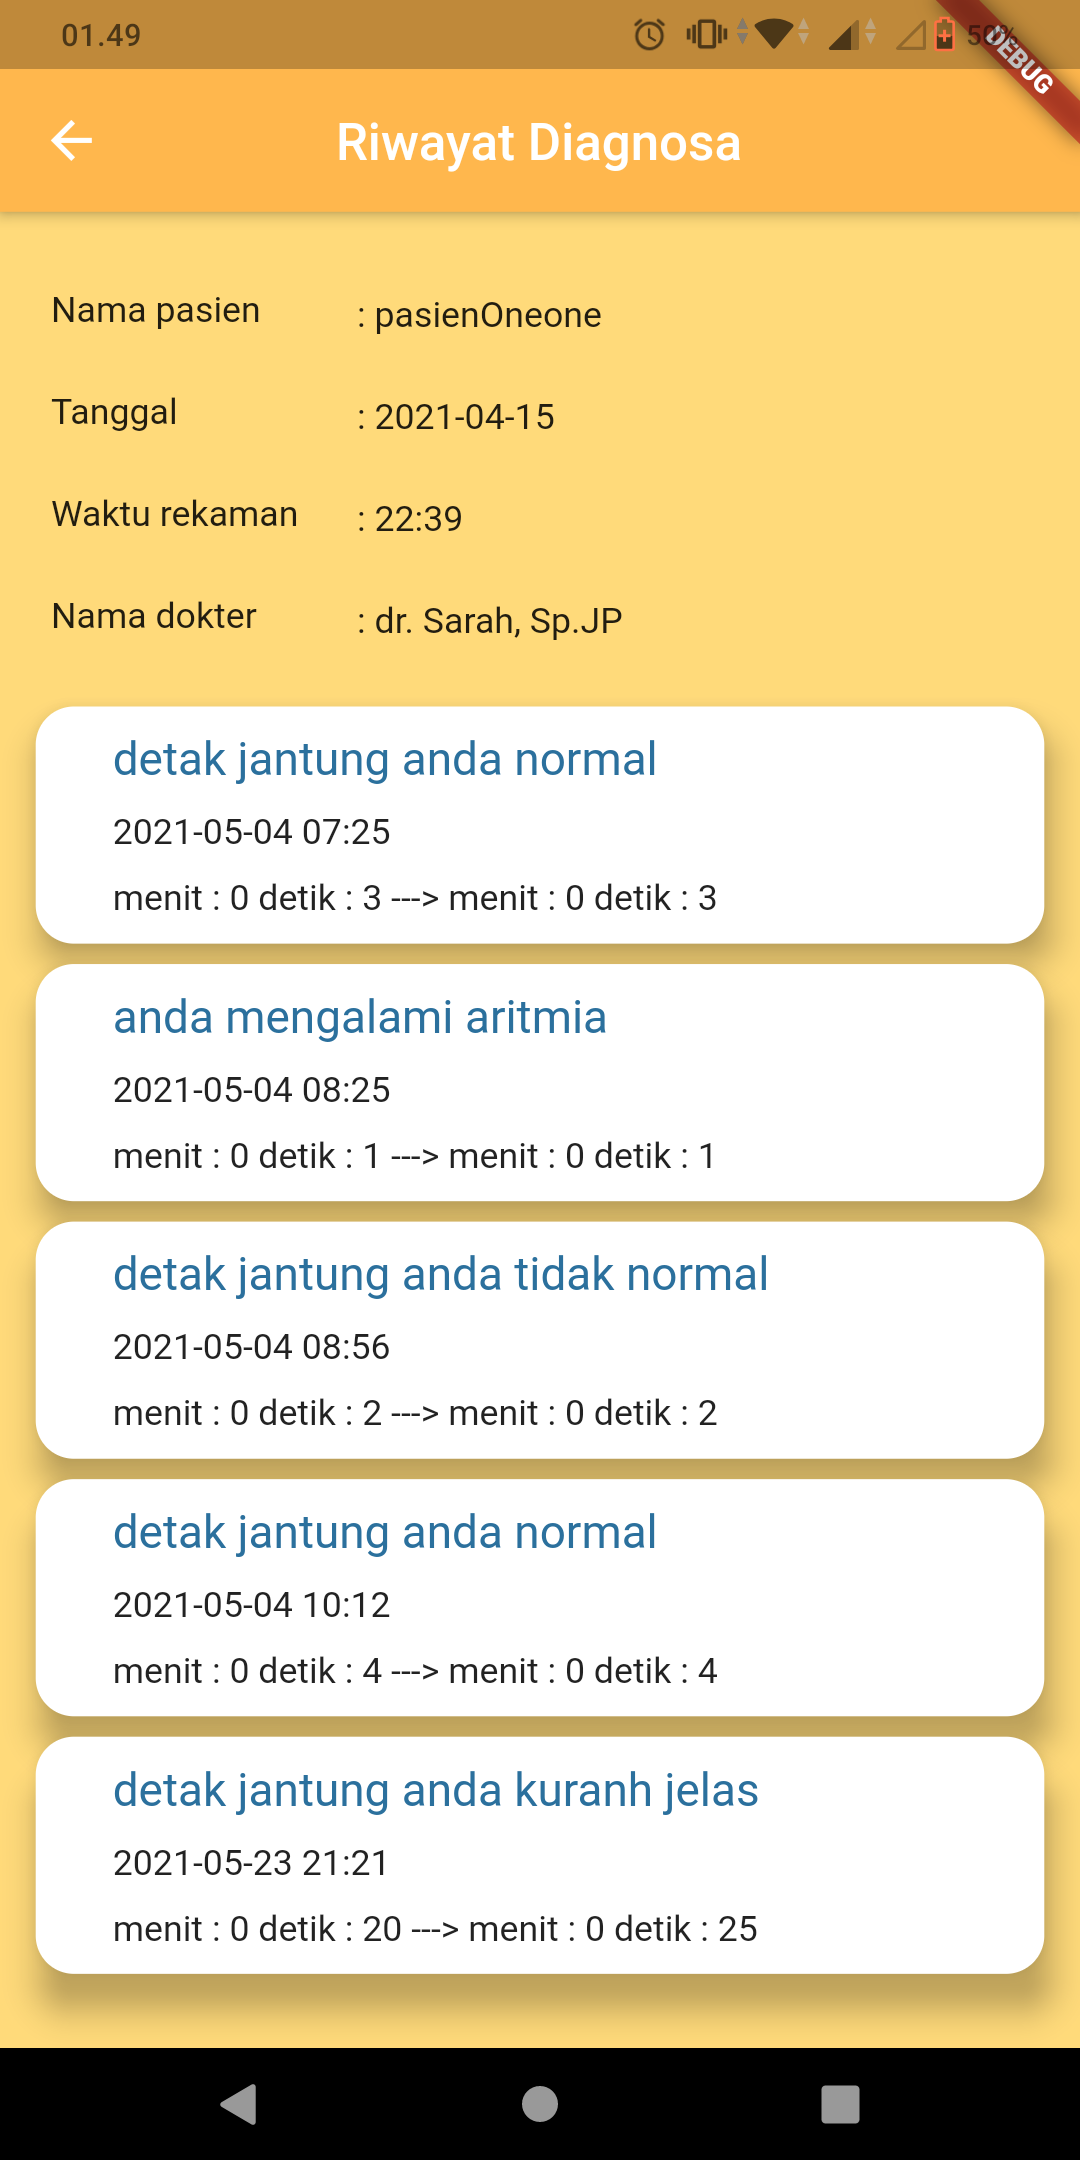
\includegraphics[width=0.2\textwidth]{img/layar_riwayatdiagnosa.png}
		\caption{Implementasi UI Riwayat Diagnosa.}
		\label{fig:3.9}
	\end{figure}
	
	\vspace{1ex}
	\subsection{Fitur Chat}
	\vspace{1ex}
	
	Pada aplikasi ini tersedia fitur chat agar pasien dapat berkonsultasi dengan dokter spesialis. Untuk cara kerja pada screen chat ini, aplikasi akan melakukan refresh setiap detik dan akan mengambil data dari database yaitu pada tabel data\_chat agar pesan terbaru pada screen chat dapat muncul. Saat mengirim pesan, pesan dari kedua user pasangan chat akan diupload pada tabel yang sama. Untuk membedakannya terdapat pada kolom id\_pengirim dan id\_penerima yang terdapat pada tabel data\_chat (Gambar \ref{fig:3.6}). Tampilan screen chat pasien dapat dilihat pada Gambar \ref{fig:3.10}.
	
	\begin{figure}[h] \centering
		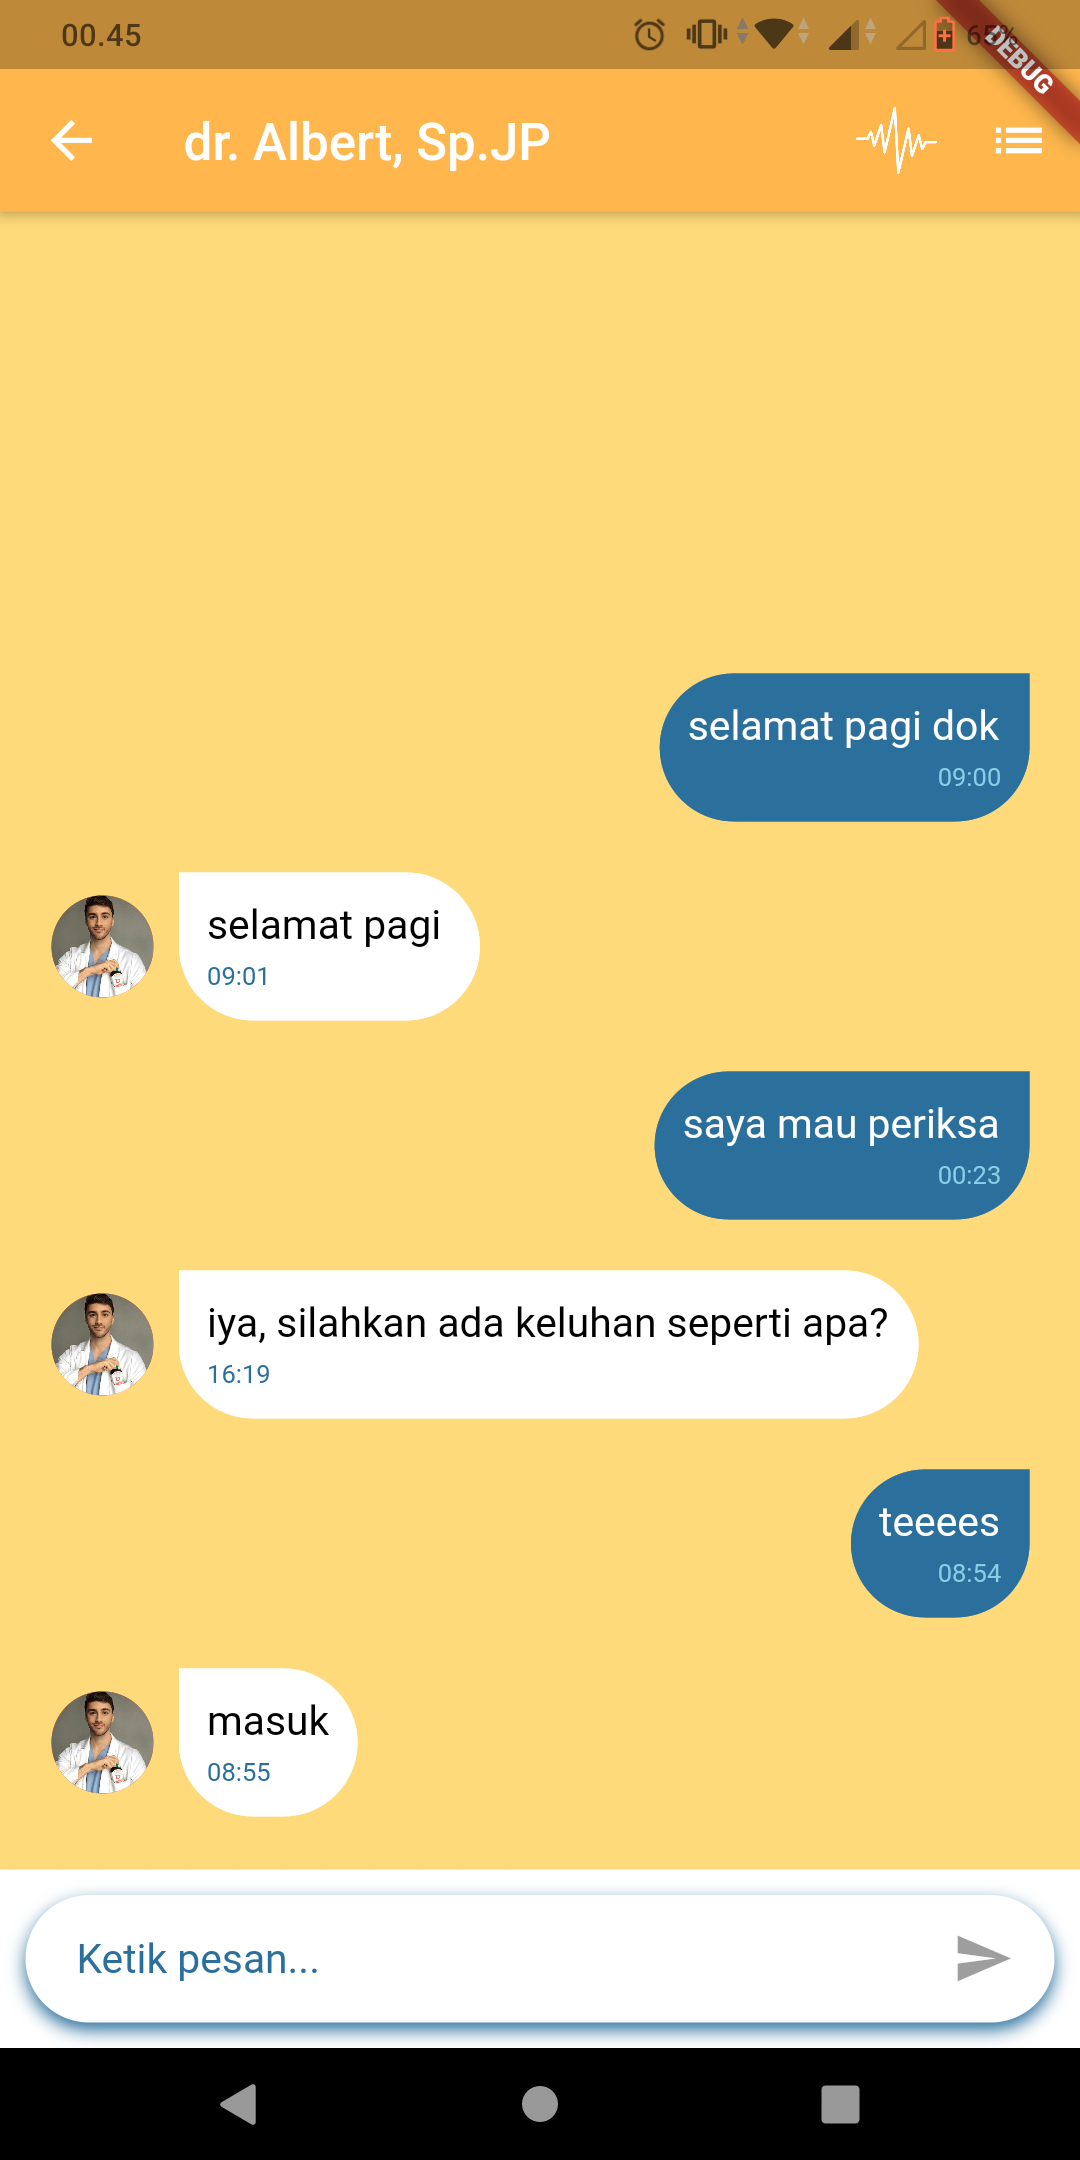
\includegraphics[width=0.2\textwidth]{img/layar_chatpasien.png}
		\caption{Implementasi UI Chatscreen Pasien.}
		\label{fig:3.10}
	\end{figure}
	
	Sedangkan untuk tampilan screen chat dokter dapat dilihat pada Gambar \ref{fig:3.11}.
	
	\begin{figure}[h] \centering
		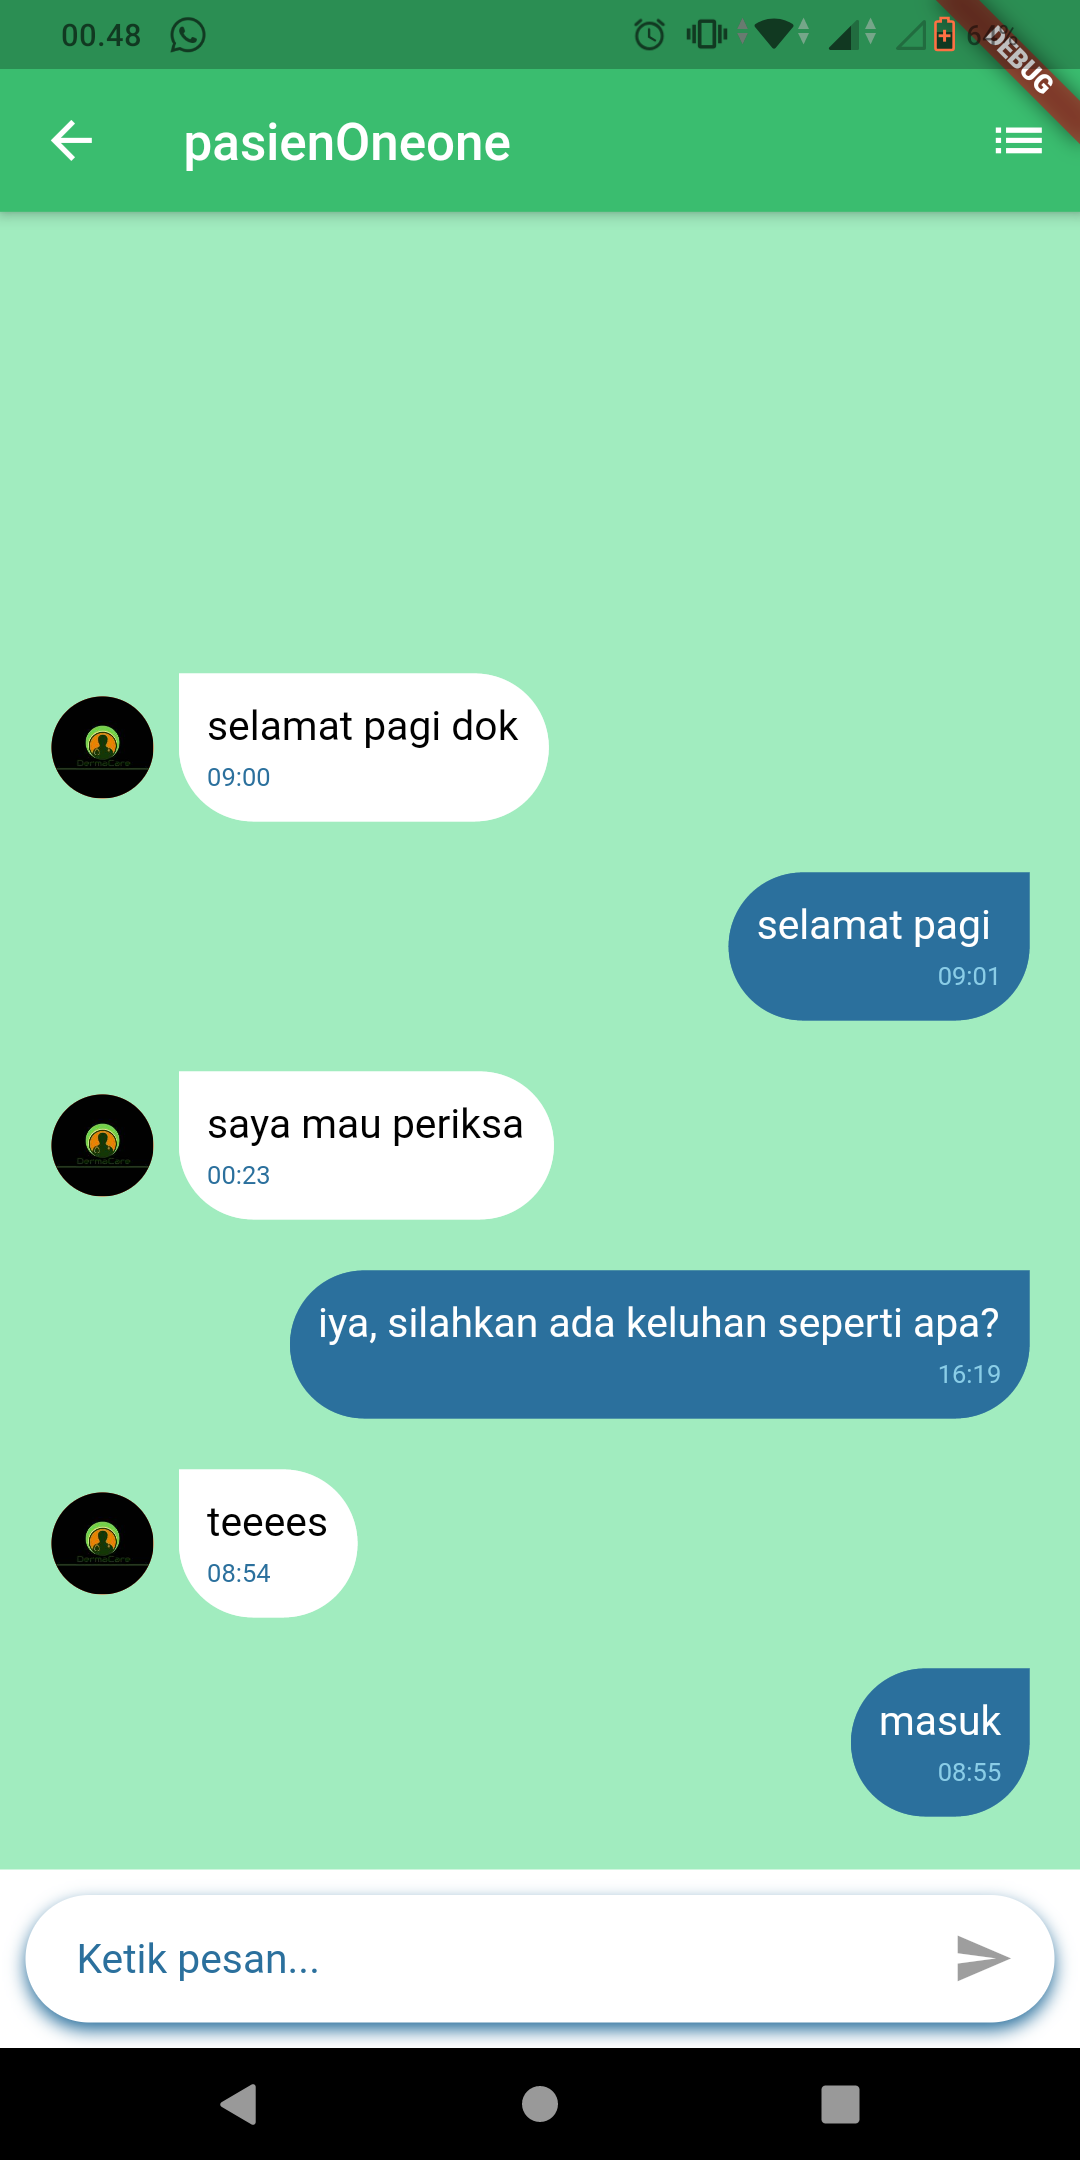
\includegraphics[width=0.2\textwidth]{img/layar_chatdokter.png}
		\caption{Implementasi UI Chatscreen Dokter.}
		\label{fig:3.11}
	\end{figure}
	
	Pada layar chat juga terdapat icon di pojok kanan atas yang berfungsi untuk jalan pintas. Pada Chatscreen pasien terdapat 2 icon yaitu icon sinyal ECG dan icon tiga garis. Icon sinyal ECG akan mengarahkan pasien menuju layar rekam data ECG sedangkan icon tiga garis akan mengarahkan pasien menuju layar riwayat rekaman ECG.
	Sedangkan pada Chatscreen dokter hanya terdapat satu icon yang akan mengarahkan dokter menuju layar riwayat rekaman ECG yang dikirimkan oleh pasien. 
	\vspace{1ex}
	
	
	\section{Pengujian dan Hasil}
	\subsection{Pengujian Frekuensi Sampling}
	\vspace{1ex}
	Pada bagian ini, pengujian dilakukan dengan cara merekam data ECG yang dikirimkan oleh arduino. Pada pengujian ini menggunakan \textit{baudrate} sebesar 9600. Pengujian ini dilakukan untuk mengetahui seberapa banyak data yang hilang dengan cara membandingkan data yang dikirim oleh mikrokontroler arduino dengan data yang diterima oleh aplikasi. Berikut adalah tabel yang merupakan hasil percobaan selama 1 menit.
	\begin{table}[h]
		\begin{tabular}{|c|c|c|c|c|c|}
			\hline
			\multicolumn{1}{|c|}{{\color[HTML]{000000} \textbf{Delay}}} & \multicolumn{1}{|c|}{\textbf{Jumlah}} &
			\multicolumn{1}{|c|}{ \textbf{Jumlah}} &
			\multicolumn{1}{|c|}{\textbf{Waktu}} &
			\multicolumn{1}{|c|}{\textbf{Frekuensi}} &
			\multicolumn{1}{|c|}{\textbf{Data}} \\
			(ms) & \textbf{Data} & \textbf{Data} & \textbf{uji} & \textbf{samplin}g & \textbf{hilang } \\
			& \textbf{dikirim} & \textbf{diterima} & (s)  &  & (\%) \\ \hline
			100 & 543 & 542 & 60 & 9.05 Hz & 0.19 \\ \hline 
			10 & 3107 & 3098 & 60 & 51.64 Hz & 0.29 \\ \hline
			5 & 4168 & 4143 & 60 & 69.05 Hz & 0.6 \\ \hline
			1 & 5748 & 5727 & 60 & 95.45 Hz & 0.37 \\ \hline
			
		\end{tabular}
		\vspace{1ex}
		\caption{Tabel hasil percobaan frekuensi sampling}
		\label{tabel:4.1}
	\end{table}
	
	Pada tabel \ref{tabel:4.1} terdapat kolom frekuensi sampling yang mana merupakan jumlah sample yang berhasil diterima oleh aplikasi dalam 1 detik. Perhitungan frekuensi sampling dengan cara perbandingan antara jumlah data diterima dengan waktu uji. Selain itu juga terdapat kolom data hilang dimana merupakan persentase jumlah data yang tidak berhasil
	diterima oleh aplikasi. Perhitungan persentase data hilang adalah dengan cara membandingkan selisih jumlah data dikirim dengan jumlah data diterima dengan jumlah data dikirim kemudian dikalikan dengan 100 \%.
	
	\vspace{1ex}
	\subsection{Pengujian Kesesuian Grafik ECG}
	\vspace{1ex}
	
	Pada tahap ini, dilakukan pengujian dengan cara membandingkan grafik ECG yang telah ditampilkan oleh aplikasi android dengan grafik ECG yang ditampilkan oleh serial ploter yang merupakan tools dari Arduino IDE. Berikut adalah hasil grafik ECG yang ditampilkan oleh aplikasi Gambar \ref{fig:4.0}.
	
	\begin{figure}[h] \centering
		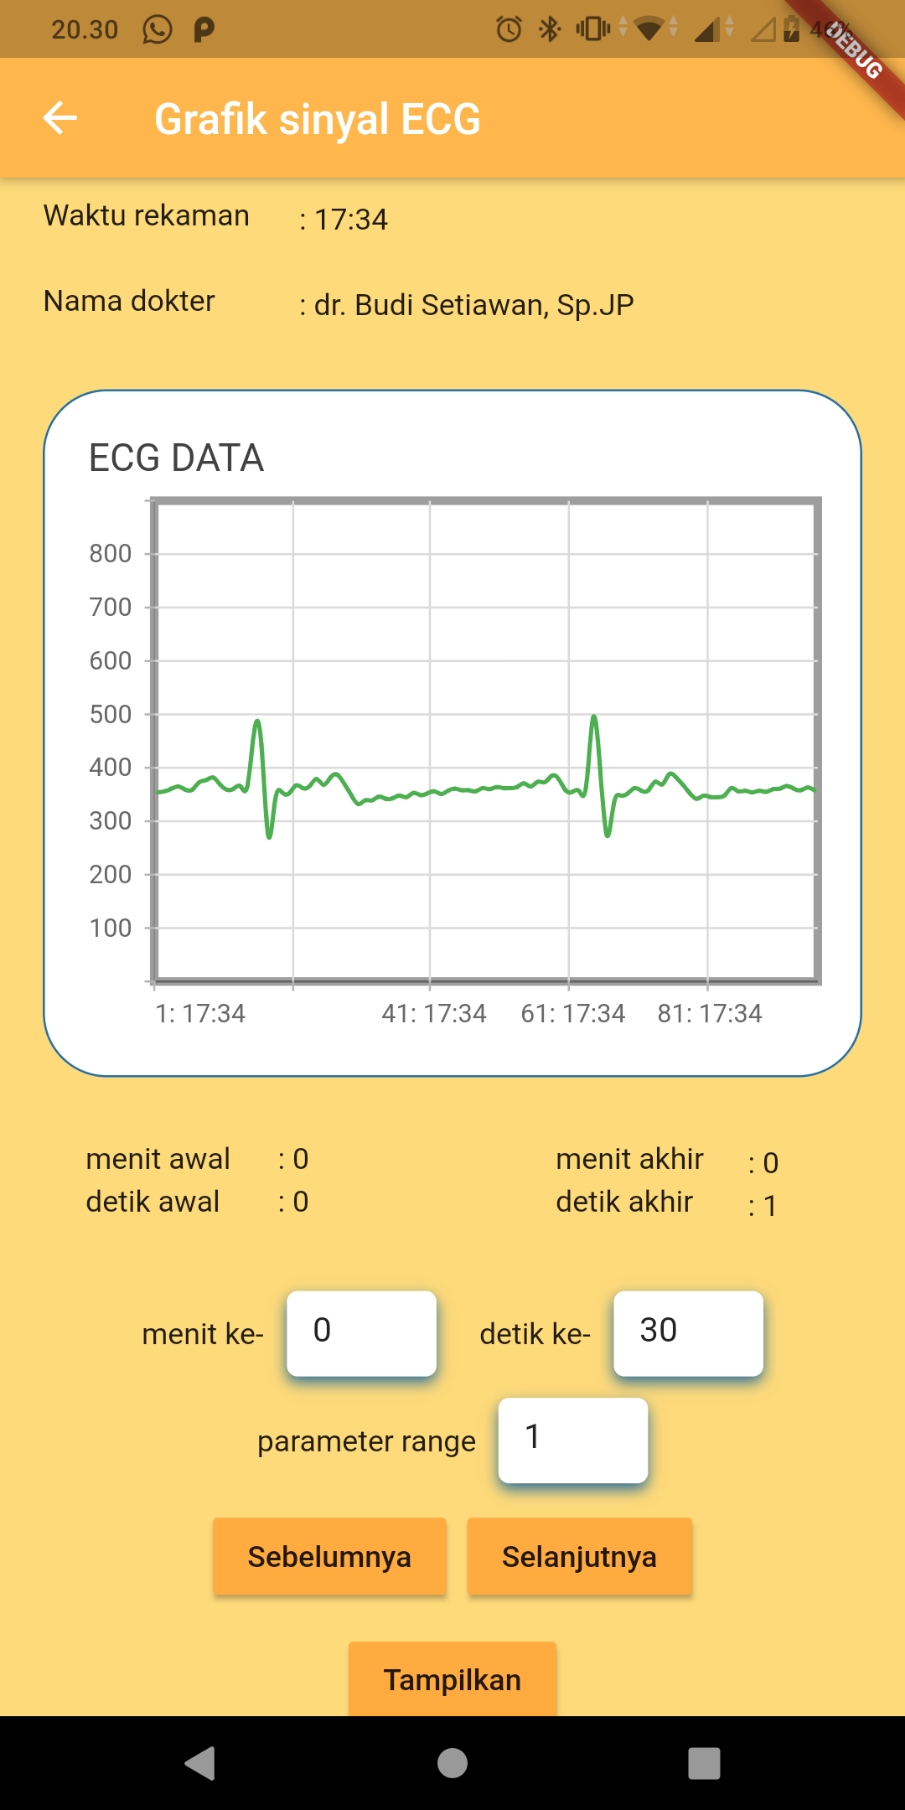
\includegraphics[width=0.25\textwidth]{img/grafikECGapps.jpg}
		\caption{Grafik ECG yang ditampilkan pada aplikasi.}
		\label{fig:4.0}
	\end{figure}
	Sedangkan grafik ECG yang ditampilkan pada serial ploter Arduino IDE ditunjukkan pada gambar berikut.
	\begin{figure}[h] \centering
		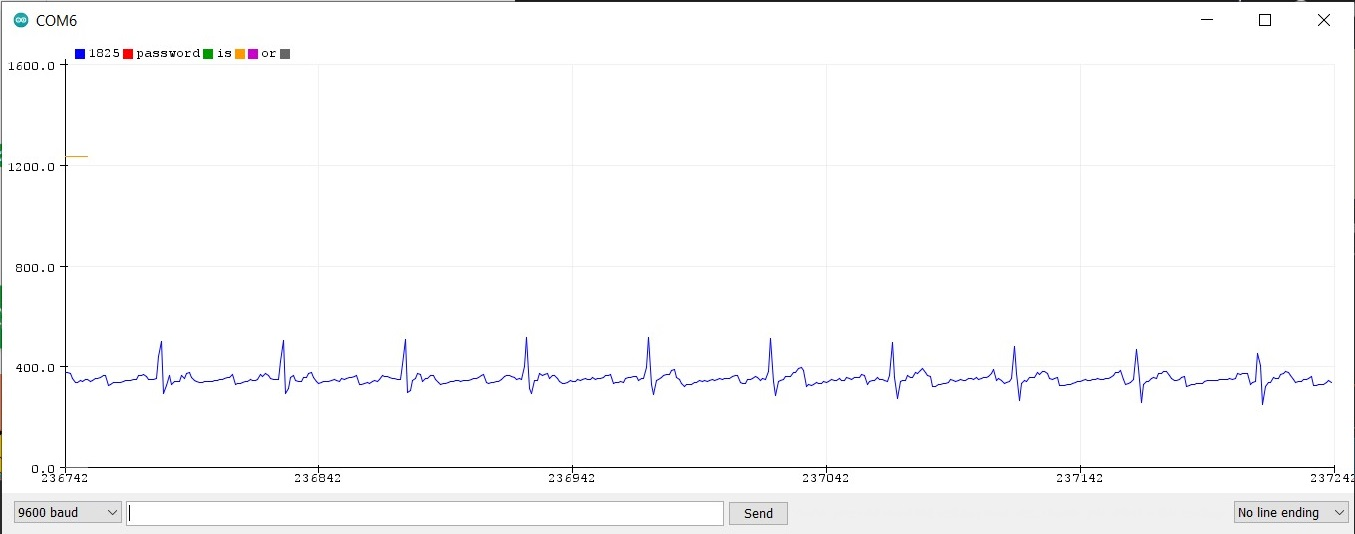
\includegraphics[width=0.45\textwidth]{img/ujisesuaidataIDE.jpg}
		\caption{Grafik ECG yang ditampilkan pada serial ploter Arduino IDE.}
		\label{fig:4.1}
	\end{figure}
	
	Berdasarkan kedua gambar diatas, apabila dibandingkan maka kedua gambar tersebut cukup mirip. Dengan demikian berarti hasil grafik ECG yang ditampilkan oleh aplikasi android cukup sesuai dengan grafik ECG yang ditampilkan oleh serial ploter Arduino IDE.
	\vspace{1ex}
	\subsection{Pengujian Waktu Pengiriman Data Menuju Database}
	\vspace{1ex}
	Pengujian ini dilakukan untuk mengetahui seberapa lama waktu yang dibutuhkan untuk mengupload data menuju database. Pengujian dilakukan dengan cara merekam data ECG secara bertahap untuk diupload yaitu dari 1 menit sampai 15 menit. Dari masing-masing tahap rekaman tersebut akan dibandingkan berapa waktu yang dibutuhkan untuk upload data.
	
	\section{Kesimpulan}
	Pada penelitian ini, dilakukan pengambilan data ECG dengan menggunakan sensor AD8232 dan kemudian dikirimkan menuju aplikasi android melalui modul bluetooth HC-05. Pengambilan data tersebut dilakukan selama 15 menit. Setelah semua data diterima oleh aplikasi, data kemudian akan diupload menuju database. Data yang telah diupload di database dapat diakses oleh Dokter Spesialis agar dapat diberi diagnosa melalui aplikasi android. Aplikasi android juga memiliki fitur chat sehingga pasien dapat berkonsultasi dengan dokter.
	
	Dari hasil pengujian yang sudah dilakukan pada bab sebelumnya, dapat ditarik beberapa kesimpulan sebagai berikut:
	Hasil pengujian untuk menghitung data yang hilang menunjukkan bahwa data yang hilang setiap sampling adalah kurang dari 1\%,	
	dari hasil pengujian kesesuaian grafik ECG menunjukkan bahwa hasil grafik ECG yang ditampilkan oleh aplikasi sudah cukup sesuai.
		
	
	\vspace{1ex}
	
	\bibliographystyle{IEEEtran}
	\bibliography{dpustaka}
\end{document}
